% ============================================================ %
%  TEMPLATE BODY                                                %
%  Styling lives in preamble.tex, per-document fields live in  %
%  metadata.tex. This file is the actual document content.     %
% ============================================================ %

\input{preamble}
% ============================================================ %
%  METADATA                                                     %
%  Edit this file per document. Everything here is the         %
%  "content" you change; the styling stays in preamble.tex.    %
% ============================================================ %

% SHOW BIBLIOGRAPHY? %
% Set to false to hide the "References" section at the end of the document.
\newtoggle{showbibliography}
\toggletrue{showbibliography}

% COVER AND HEADER FIELDS %
\newcommand{\doctitle}{2110413 COMPUTER SECURITY}
\newcommand{\docauthor}{Worralop Srichainont}
\newcommand{\docdate}{\today}
\newcommand{\coursecode}{2110413}
\newcommand{\coursename}{COMPUTER SECURITY}
\newcommand{\assignmentname}{Log Analysis}
\newcommand{\institution}{Computer Engineering, Chulalongkorn University}
\newcommand{\assignmentnumber}{2}
\newcommand{\instructor}{Instructor Name}
\newcommand{\studentid}{6632200221}
\newcommand{\duedate}{\today}


% PDF METADATA AND LINK STYLING (needs the fields from metadata.tex) %
\definecolor{linkaccent}{HTML}{1a56db}
\hypersetup{
    pdftitle={\doctitle},
    pdfauthor={\docauthor},
    pdfsubject={\coursecode\ -- \coursename},
    colorlinks=true,
    linkcolor=linkaccent,
    citecolor=linkaccent,
    urlcolor=linkaccent,
    bookmarksnumbered=true,
}

% Drop the automatic "N.N" subsection number from the running header mark
% (\rightmark) so long subsection titles don't collide with the course-code
% header on the left; the number still prints normally in the heading itself.
\renewcommand{\subsectionmark}[1]{\markright{#1}}

% DOCUMENT CONTENTS %
\begin{document}

    % ======================================================== %
    % COVER PAGE                                                %
    % ======================================================== %
    \begin{titlepage}
        \centering
        \thispagestyle{empty}
        \vspace*{4em}

        {\scshape Assignment}

        \vspace{3em}
        {\Huge\bfseries \doctitle}
        \vspace{1.5em}

        \noindent\rule{0.6\textwidth}{0.5pt}
        \vspace{1.5em}

        {\large Assignment \assignmentnumber} \\[0.4em]
        {\large \assignmentname}

        \vfill

        {\large \institution}
        \vspace{1em}

        {\large \docauthor}

        \vspace{0.4em}
        {\normalsize Student ID: \studentid}

        % \vspace{1.5em}
        % {\normalsize Instructor: \instructor \quad\textbar\quad Due: \duedate}

        \vspace{2em}
        {\normalsize \docdate}
    \end{titlepage}

    % ======================================================== %
    % TABLE OF CONTENTS                                         %
    % ======================================================== %
    \tableofcontents
    \thispagestyle{empty}
    \clearpage

    % ======================================================== %
    % BODY (running header/footer active from here on)          %
    % ======================================================== %
    \pagenumbering{arabic}

    \section{Introduction}

        For this assignment, we act as a member of the security/incident management team of a company named
        buttercup. The company's infrastructure consists of a mail server \texttt{mailsv} and three web servers
        \texttt{www1}, \texttt{www2}, \texttt{www3}. We are given the \texttt{secure.log} (authentication) and
        \texttt{access.log} (web access) files from these servers, and our job is to find out whether anyone is
        trying to hack, scan, or access protected information on them. Reading these logs line by line would be
        painful, so instead of writing our own parsing code, we use \textbf{Splunk} to search and aggregate the
        data.

        We already imported the provided \texttt{tutorialdata.zip} into Splunk as a single upload (so every event
        is indexed exactly once), and every search below is run with the time range set to \textbf{All time}, since
        the events are not from the last 24 hours.

    \section{Part I: Suspicious Login Activity}

        On Linux servers, \texttt{secure.log} contains the authentication events, so this is where we look first
        to see if someone is trying to log in to a server they should not.

        \subsection[Hackers]{Q1: How Many Hackers, How Many Attempts}

            \begin{defbox}[Definition: hacker and attempt]
                We define a \textbf{hacker} as a distinct source IP address that produced at least one
                \texttt{Failed password} line in \texttt{secure.log}. Each such line is counted as one
                \textbf{attempt}. This way, one hacker trying 200 times is still one hacker, but contributes 200
                attempts.
            \end{defbox}

            To count them, we search for \texttt{Failed password} lines, extract the source IP with \texttt{rex},
            then count the distinct IPs and the total number of matching lines.

            \begin{codeblock}{text}{Count Distinct Attackers}
                source="*secure.log" "Failed password"
                | rex "from (?<src_ip>\S+) port"
                | stats dc(src_ip) as distinct_hackers count as attempts
            \end{codeblock}

            \begin{figure}[h]
                \centering
                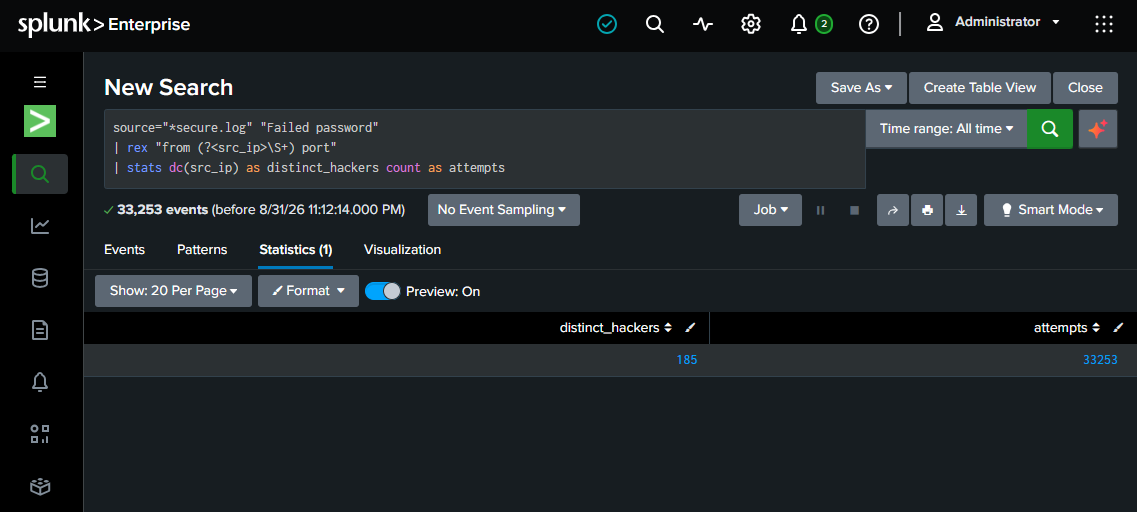
\includegraphics[width=0.9\linewidth]{images/q1.png}
                \caption{Distinct attacking IP addresses and total failed-password attempts.}
                \label{fig:q1}
            \end{figure}

            \Cref{fig:q1} shows that there are \textbf{185} distinct source IPs, so we count \textbf{185 hackers}
            trying to get access to our servers, with \textbf{33,253 attempts} in total.

        \subsection[Attack Time]{Q2: What Time Do Hackers Appear}

            We bucket every \texttt{Failed password} event by hour of day and count how many attempts fall in
            each bucket.

            \begin{codeblock}{text}{Attempts by Hour}
                source="*secure.log" "Failed password"
                | eval hour=strftime(_time, "%H:00-%H:59")
                | stats count as attempts by hour
                | sort - attempts
            \end{codeblock}

            \begin{figure}[h]
                \centering
                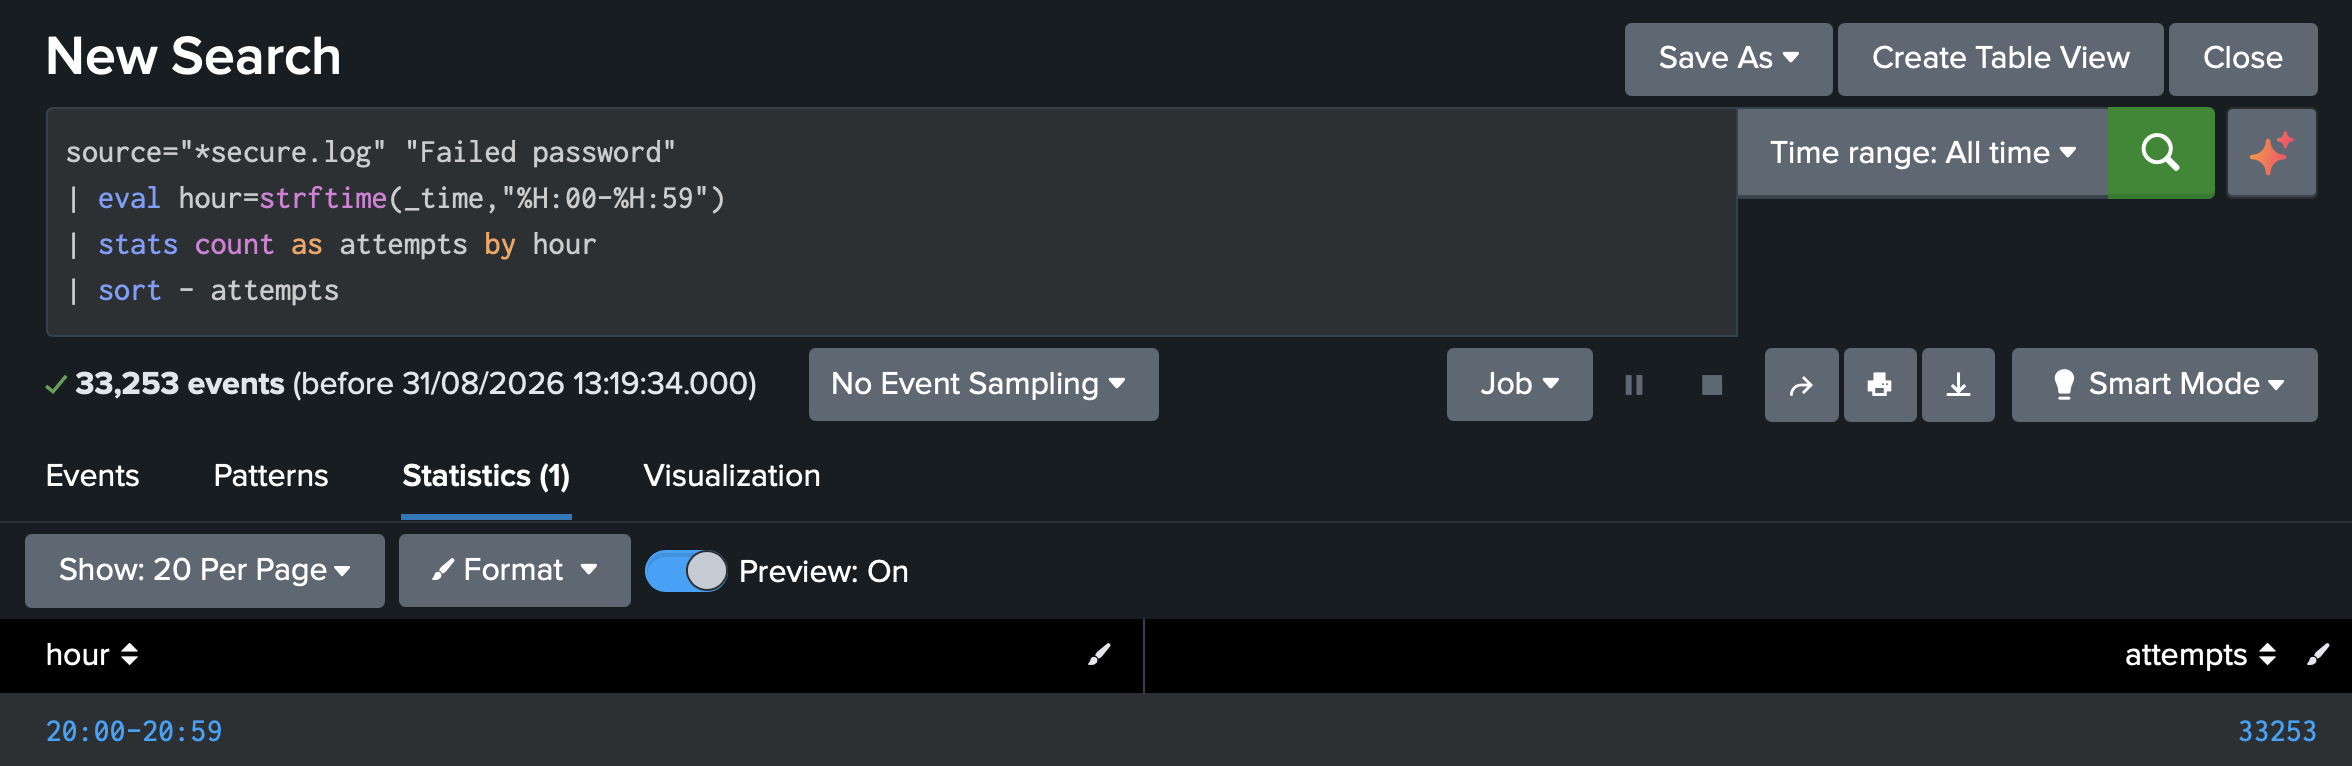
\includegraphics[width=0.9\linewidth]{images/q2.png}
                \caption{Failed-password attempts grouped by hour of day.}
                \label{fig:q2}
            \end{figure}

            \Cref{fig:q2} shows all 33,253 attempts falling into a single hour bucket, \textbf{20:00--20:59}. So,
            based on this data, hackers appear to try to hack our servers during the \textbf{20:00--20:59} hour.

        \subsection[Busiest Server]{Q3: Which Server Had the Most Attempts}

            \begin{notebox}[Note: the \texttt{host} field is not reliable here]
                Our first instinct was to group by Splunk's \texttt{host} field, since we set the input to use
                ``Segment in path'' when uploading the data. This did not work as expected.
            \end{notebox}

            \begin{codeblock}{text}{Attempts by Host (does not work)}
                source="*secure.log" "Failed password"
                | stats count as attempts by host
                | sort - attempts
            \end{codeblock}

            \begin{figure}[h]
                \centering
                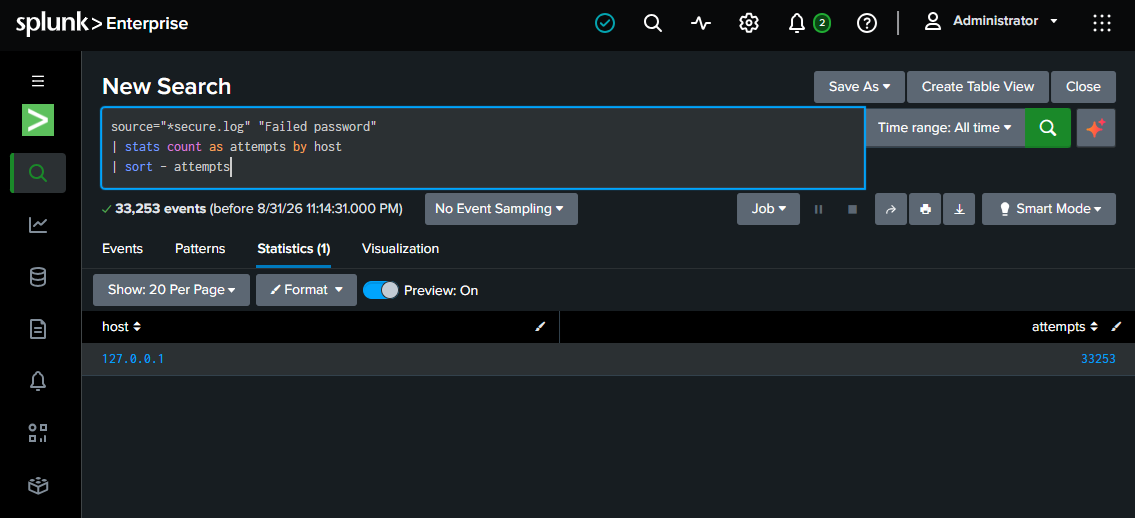
\includegraphics[width=0.9\linewidth]{images/q3-2.png}
                \caption{Grouping by \texttt{host} puts every event under a single \texttt{127.0.0.1} host.}
                \label{fig:q3-2}
            \end{figure}

            \Cref{fig:q3-2} shows all 33,253 events under one host, \texttt{127.0.0.1}, which is just the machine
            we uploaded the data from, not the actual server name. So instead of relying on \texttt{host}, we
            parse the server name straight out of the \texttt{source} file path with \texttt{rex}.

            \begin{codeblock}{text}{Attempts by Server}
                source="*secure.log" "Failed password"
                | rex field=source "/(?<server>mailsv|www1|www2|www3)/secure\.log"
                | stats count as attempts by server
                | sort - attempts
            \end{codeblock}

            \begin{figure}[h]
                \centering
                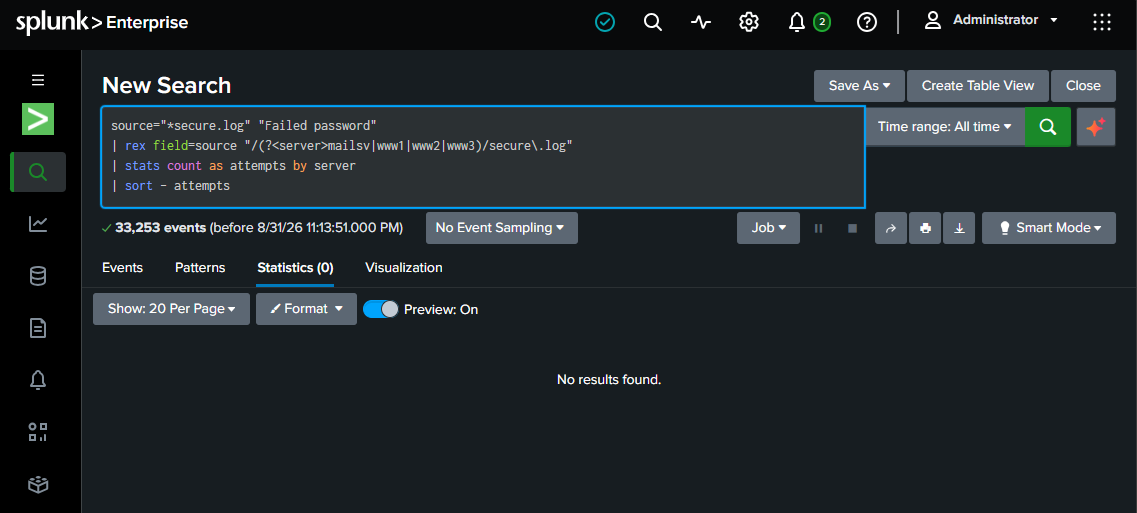
\includegraphics[width=0.9\linewidth]{images/q3-1.png}
                \caption{Failed-password attempts grouped by server, parsed from the source path.}
                \label{fig:q3-1}
            \end{figure}

            \Cref{fig:q3-1} shows \textbf{www1} with 8,798 attempts, ahead of www3 (8,267), mailsv (8,154), and
            www2 (8,034). So \textbf{www1} had the most attempts.

            \begin{takeawaybox}
                www1 is the server under the heaviest brute-force pressure, but the difference across the four
                servers is small; attackers are not favoring one server much over the others.
            \end{takeawaybox}

        \subsection[Top Account]{Q4: Most Popular Account}

            We extract the account name from the same \texttt{Failed password} lines and take the top 5 by
            attempt count.

            \begin{codeblock}{text}{Top Attempted Accounts}
                source="*secure.log" "Failed password"
                | rex "Failed password for (?:invalid user )?(?<account>\S+) from"
                | stats count as attempts by account
                | sort - attempts
                | head 5
            \end{codeblock}

            \begin{figure}[h]
                \centering
                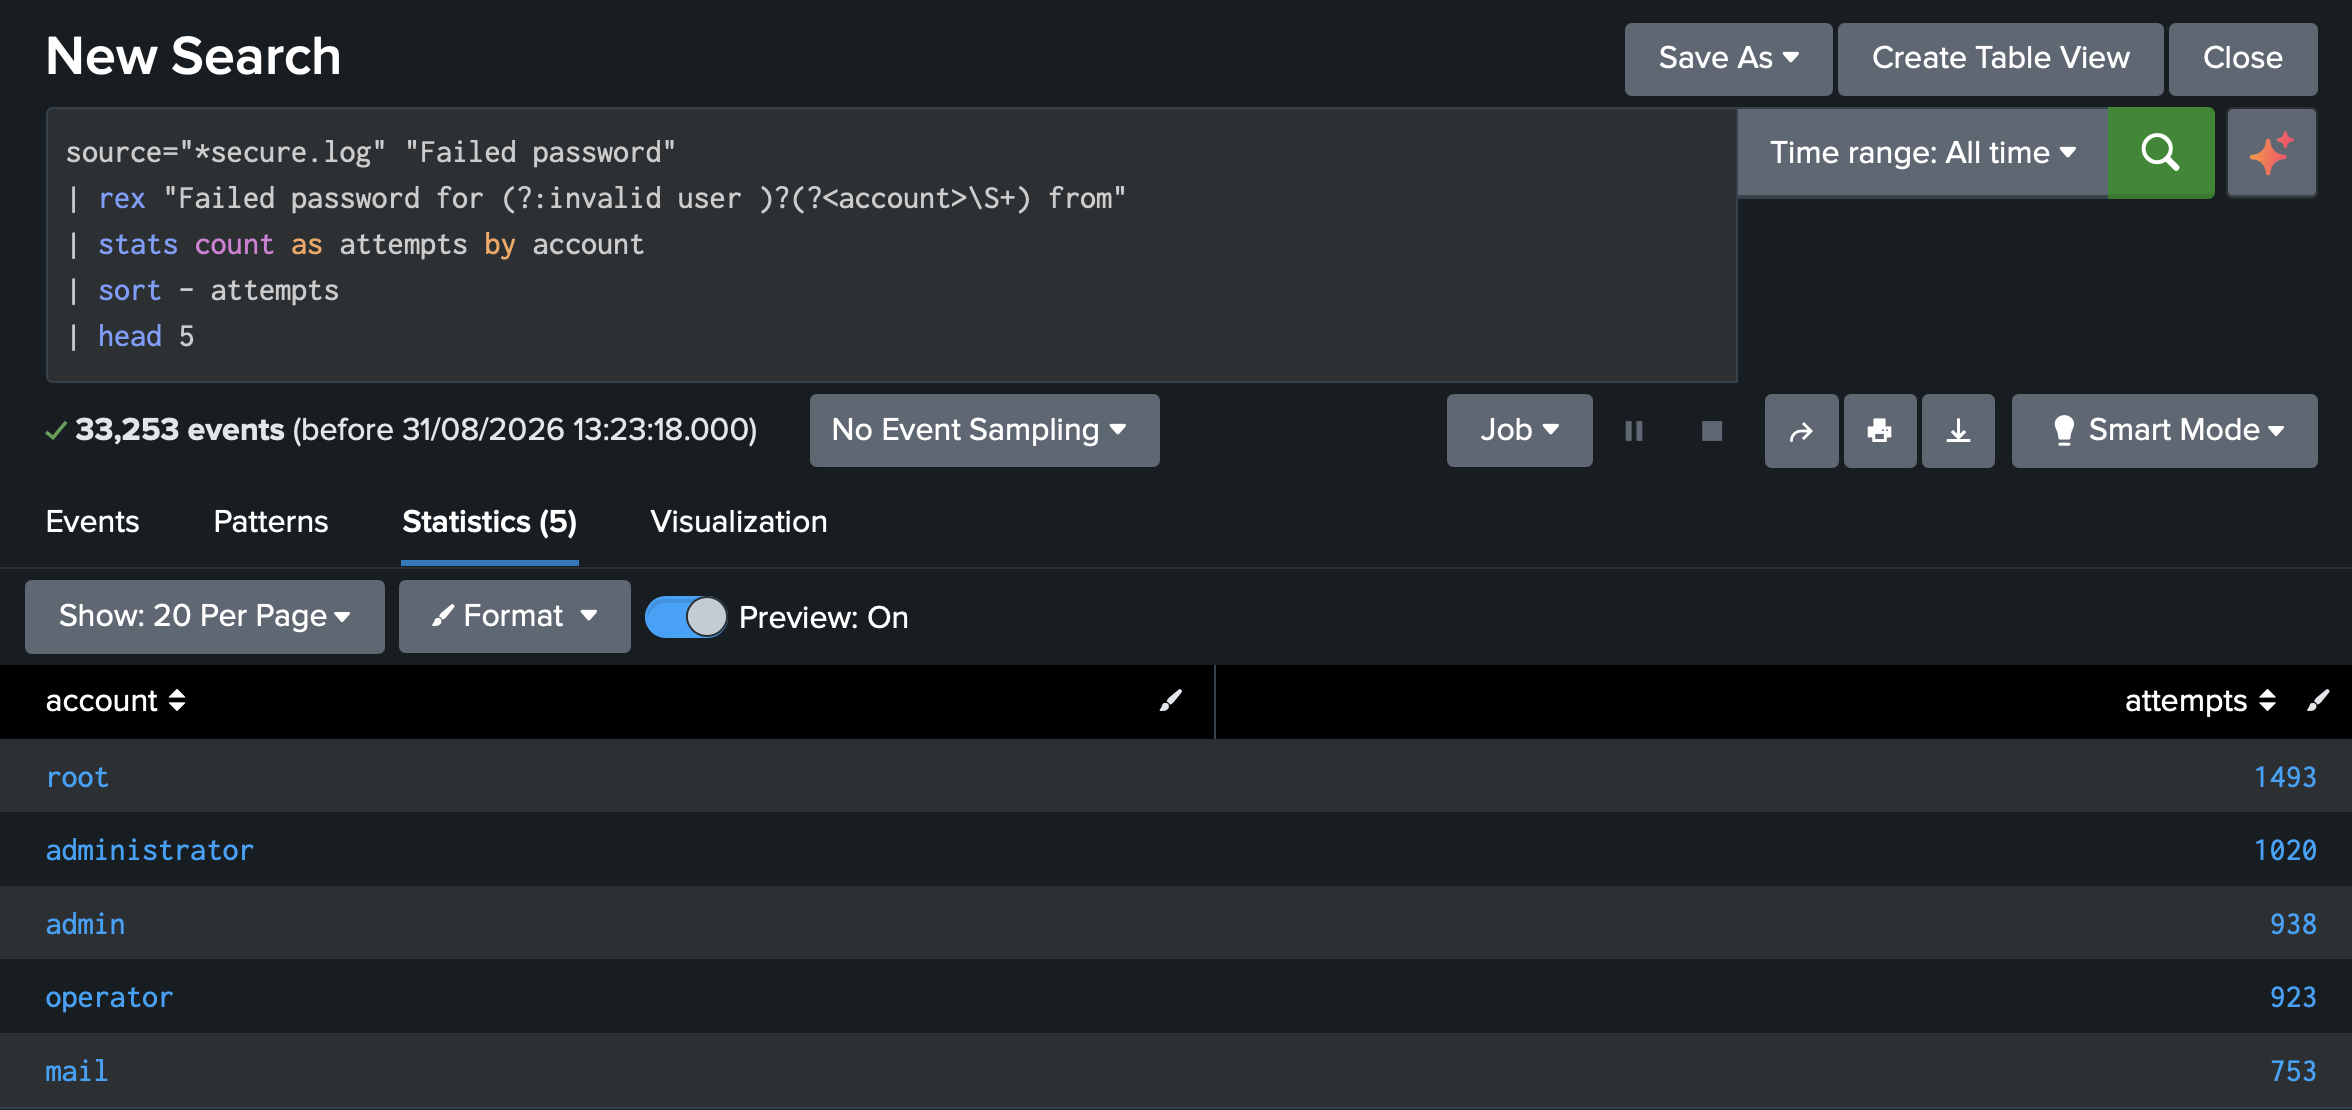
\includegraphics[width=0.9\linewidth]{images/q4.png}
                \caption{Top 5 account names used in failed-password attempts.}
                \label{fig:q4}
            \end{figure}

            \Cref{fig:q4} shows \textbf{root} as the most popular account (1,493 attempts), followed by
            administrator (1,020), admin (938), operator (923), and mail (753). Hackers are mostly guessing
            generic admin-sounding usernames rather than real people's accounts.

    \section{Part II: Sensitive Files on Web Servers}

        On web servers, \texttt{access.log} contains the web access events. Following the
        \href{https://zeltser.com/security-incident-log-review-checklist/}{security incident log review checklist},
        we look for excessive access attempts to non-existent files and error code 404 on files that are not
        part of our actual shop.

        \begin{notebox}[Note: what we are looking for]
            The checklist for web servers specifically calls out ``excessive access attempts to non-existent
            files'' and ``access to extensions you have not implemented''. In this data set, we found four such
            paths, all returning \textbf{404}: \texttt{/passwords.pdf}, \texttt{/hidden/anna\_nicole.html},
            \texttt{/rush/signals.zip}, and \texttt{/numa/numa.html}. None of these belong to the real
            \texttt{buttercupgames.com} storefront, which only serves \texttt{/cart.do}, \texttt{/product.screen},
            \texttt{/category.screen}, and similar pages.
        \end{notebox}

        \subsection[Sensitive Files]{Q5: Attempts to Access Sensitive Information}

            First, we count how many times any of the four suspicious paths were requested.

            \begin{codeblock}{text}{Count Sensitive-Path Probes}
                source="*access.log" ("/passwords.pdf" OR "/hidden/" OR "/rush/signals.zip" OR "/numa/numa.html")
                | stats count as attempts
            \end{codeblock}

            \begin{figure}[h]
                \centering
                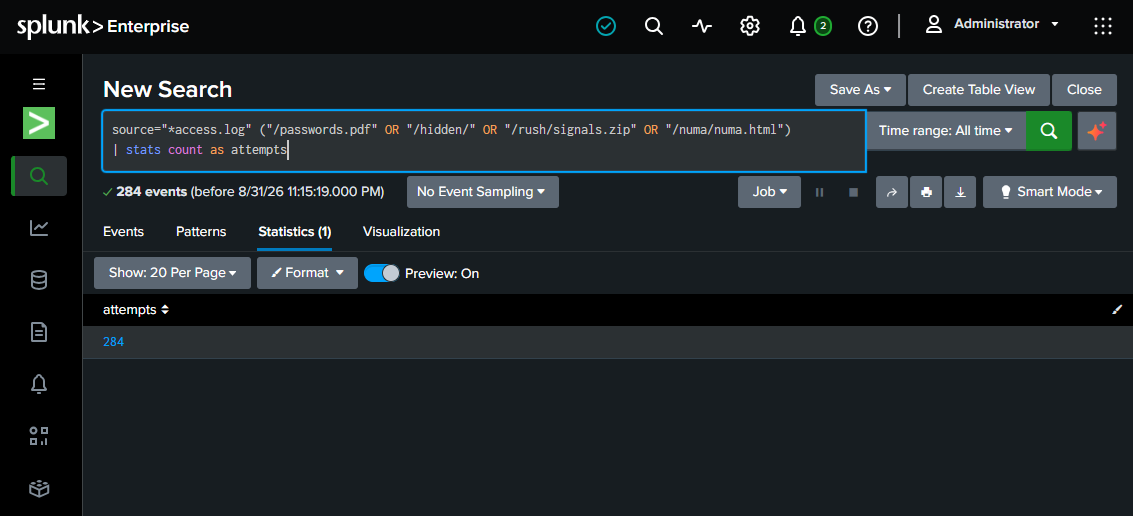
\includegraphics[width=0.9\linewidth]{images/q5-1.png}
                \caption{Total attempts to access the four suspicious paths.}
                \label{fig:q5-1}
            \end{figure}

            \Cref{fig:q5-1} shows \textbf{284} attempts. As broader supporting evidence, we also look at every
            404 response on the web servers, not just our four suspicious paths.

            \begin{codeblock}{text}{All 404 Paths}
                source="*access.log" status=404
                | stats count by uri_path
                | sort - count
            \end{codeblock}

            \begin{figure}[h]
                \centering
                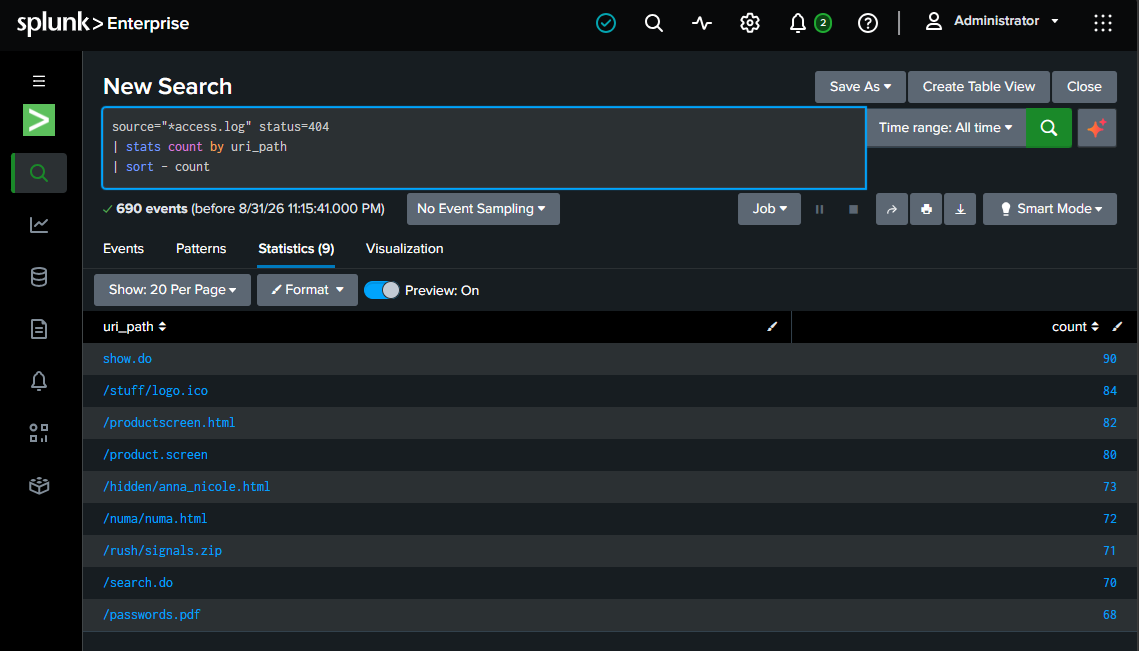
\includegraphics[width=0.9\linewidth]{images/q5-2.png}
                \caption{Every path that returned a 404, sorted by count.}
                \label{fig:q5-2}
            \end{figure}

            \Cref{fig:q5-2} shows 690 total 404 events across all paths, with our four suspicious paths
            (\texttt{/hidden/anna\_nicole.html}, \texttt{/numa/numa.html}, \texttt{/rush/signals.zip},
            \texttt{/passwords.pdf}) all sitting near the top of the list. So yes, we can find attempts to get
            access to sensitive information, and there were \textbf{284} such attempts.

        \subsection[Targeted Files]{Q6: What Resource Are Hackers Looking For}

            \begin{codeblock}{text}{Sensitive-Path Probes by File}
                source="*access.log" ("/passwords.pdf" OR "/hidden/" OR "/rush/signals.zip" OR "/numa/numa.html")
                | stats count as attempts by uri_path
                | sort - attempts
            \end{codeblock}

            \begin{figure}[h]
                \centering
                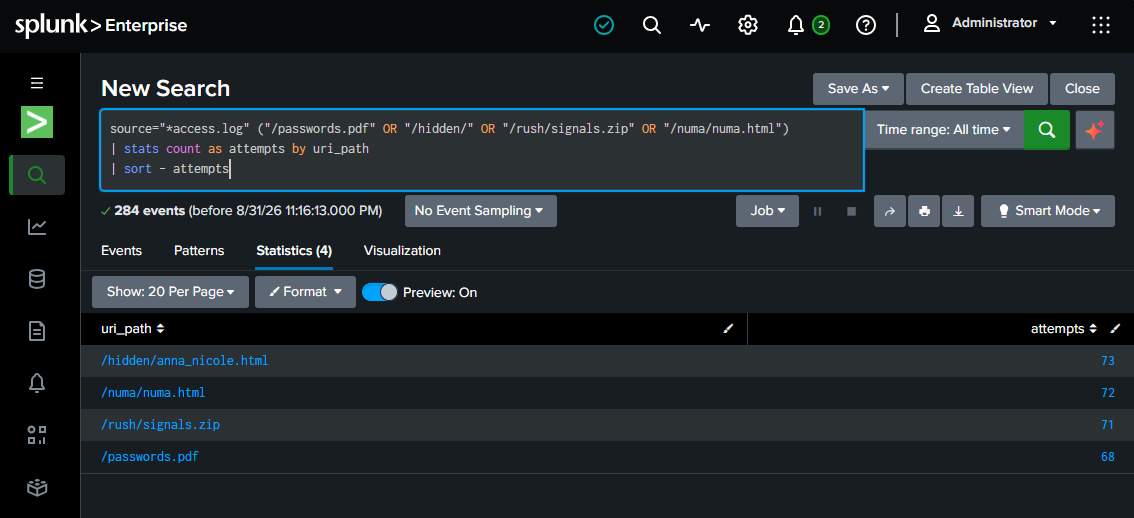
\includegraphics[width=0.9\linewidth]{images/q6.png}
                \caption{Attempts broken down by the specific file requested.}
                \label{fig:q6}
            \end{figure}

            \Cref{fig:q6} breaks the 284 attempts down by file: \texttt{/hidden/anna\_nicole.html} (73),
            \texttt{/numa/numa.html} (72), \texttt{/rush/signals.zip} (71), and \texttt{/passwords.pdf} (68).

            \begin{takeawaybox}
                All four files are being probed at almost the same rate, but \texttt{passwords.pdf} is the
                clearest sensitive-information target by name; the others read more like an attacker fishing for
                any interesting-looking file on the server.
            \end{takeawaybox}

    \section{Part III: Are There Bots Crawling Our Websites}

        \subsection[Finding Bots]{Q7: Finding Bots}

            The hint tells us to look at the \texttt{User-Agent} field in \texttt{access.log}. We first try
            filtering directly on Splunk's extracted \texttt{useragent} field.

            \begin{codeblock}{text}{Bots via useragent Field}
                source="*access.log" (useragent="*bot*" OR useragent="*Bot*" OR useragent="*crawler*" OR useragent="*Netcraft*")
                | stats count as hits by useragent
                | sort - hits
            \end{codeblock}

            \begin{figure}[h]
                \centering
                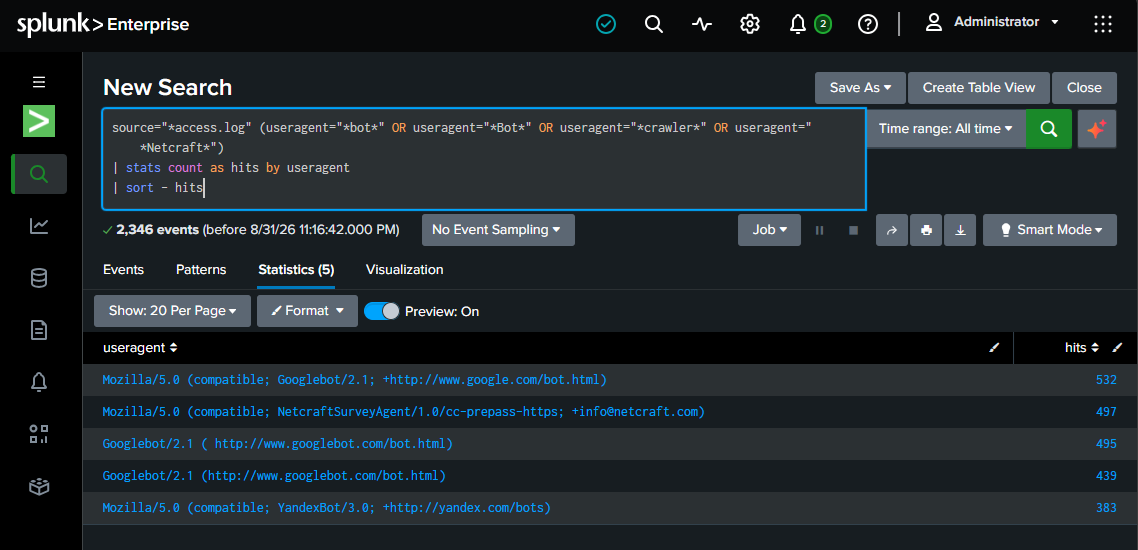
\includegraphics[width=0.9\linewidth]{images/q7-1.png}
                \caption{Requests grouped by bot-like user agent, using the extracted field.}
                \label{fig:q7-1}
            \end{figure}

            As a cross-check, we also match on the raw event text and re-extract the user agent with \texttt{rex},
            in case the \texttt{useragent} field was not extracted the same way for every event.

            \begin{codeblock}{text}{Bots via Raw-Text rex Fallback}
                source="*access.log" ("Googlebot" OR "YandexBot" OR "NetcraftSurveyAgent")
                | rex "\"(?<ua>[^\"]+)\"\s+\d+\s*$"
                | stats count as hits by ua
                | sort - hits
            \end{codeblock}

            \begin{figure}[h]
                \centering
                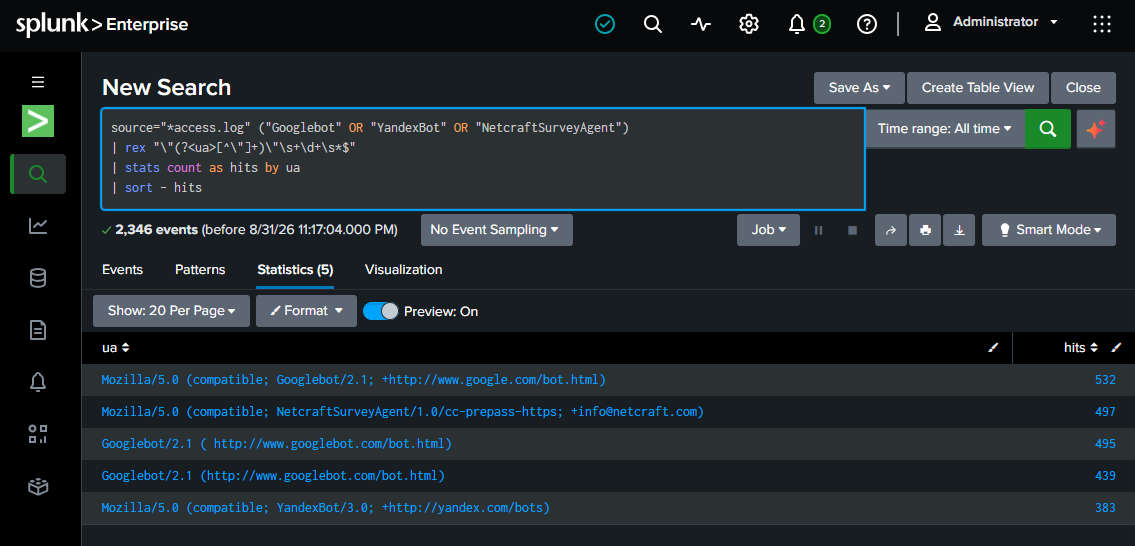
\includegraphics[width=0.9\linewidth]{images/q7-2.png}
                \caption{Same bot traffic, re-extracted directly from the raw event text.}
                \label{fig:q7-2}
            \end{figure}

            Both \cref{fig:q7-1} and \cref{fig:q7-2} agree on the same 2,346 events and the same top 5 user
            agents, so we are confident the field extraction is correct. So yes, we can find bots crawling our
            websites: \textbf{Googlebot} (three different user-agent strings, 532/495/439 hits), the
            \textbf{NetcraftSurveyAgent} (497 hits), and \textbf{YandexBot} (383 hits).

        \subsection[Bot Behavior]{Q8: What Are the Bots Doing}

            \begin{codeblock}{text}{Bot Activity by Path and Status}
                source="*access.log" ("Googlebot" OR "YandexBot" OR "NetcraftSurveyAgent")
                | stats count as hits by uri_path, status
                | sort - hits
            \end{codeblock}

            \begin{figure}[h]
                \centering
                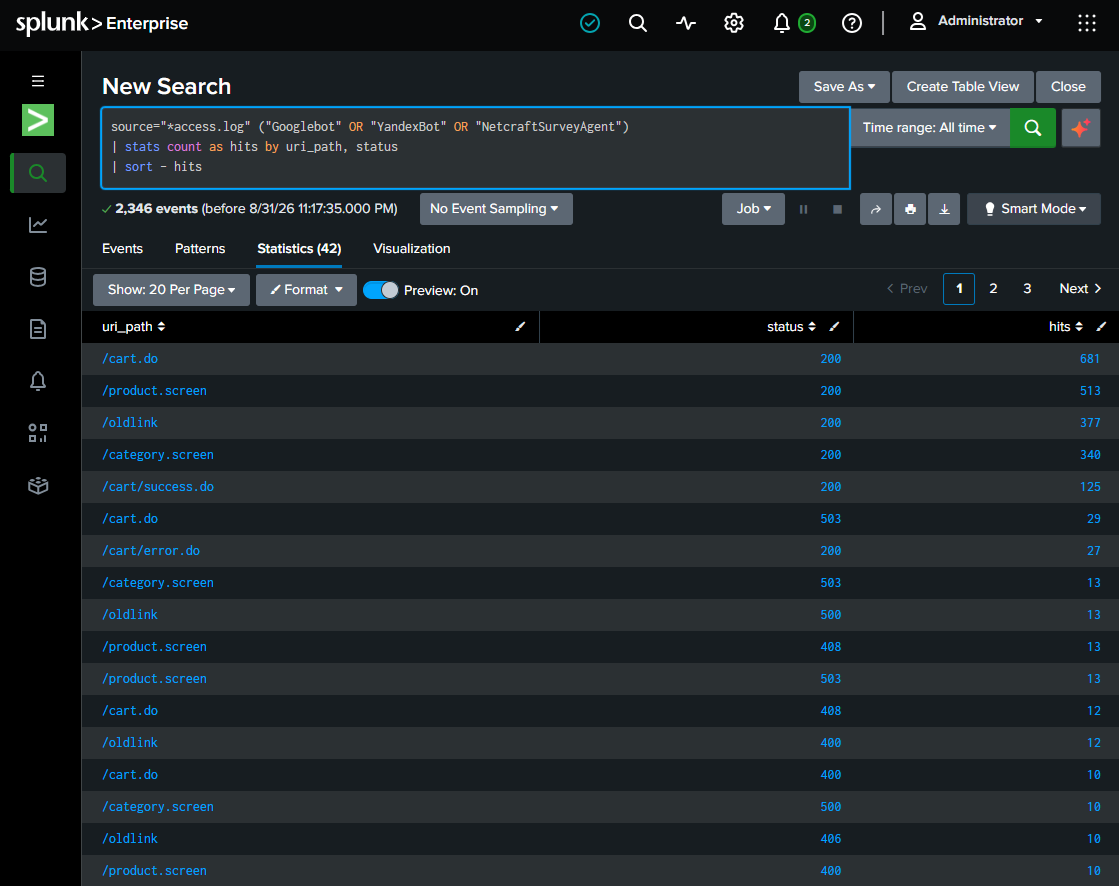
\includegraphics[width=0.9\linewidth]{images/q8.png}
                \caption{Bot traffic broken down by requested path and HTTP status.}
                \label{fig:q8}
            \end{figure}

            \Cref{fig:q8} shows the bots mostly browsing the same storefront pages a normal shopper would:
            \texttt{/cart.do} (681), \texttt{/product.screen} (513), \texttt{/oldlink} (377),
            \texttt{/category.screen} (340), and \texttt{/cart/success.do} (125), almost all with status 200.
            Only a small number of hits land on error statuses (503, 500, 408, 406, 400) on those same pages.

            \begin{takeawaybox}
                The bot traffic we see (Googlebot, YandexBot, NetcraftSurveyAgent) is legitimate search-engine
                and monitoring crawling, not an attack; it walks the normal product catalog the same way a
                shopper would, unlike the sensitive-path probing in Part II.
            \end{takeawaybox}

\end{document}
